% 原典 PDF pp.305--327（原書 pp.283--305）、第9章導入・9.1--9.4。
\sectionlink{高次の振幅}\label{ch:9}
本章では弦理論の高次の振幅を論じる。前半の主な目標は、弦の摂動論の有限性とユニタリティを理解することである。ツリーレベルの振幅をある程度詳しく調べたのち、因子化の考えを用いて高次の振幅と低次の振幅を関係づけながら、一般的な振幅を考察する。後半では、全次数、さらには非摂動的な弦理論を理解するために提案されてきたいくつかの考えを簡潔に論じる。超対称性に基づく、より強力な方法は第2巻まで扱わない。本章は本書の主な展開から外れているので、最初に読む際には飛ばしてもよい。

\subsectionlink{一般のツリーレベル振幅}\label{sec:9.1}
第6章では、主としていくつかの具体的なツリーレベル振幅の計算を扱った。本章を一般のツリー振幅の解析から始めると、高次の振幅にも現れるいくつかの構造がわかって有用である。向き付けられた閉弦に焦点を絞り、重要な特徴を示す3点および4点振幅を考える。主な問題は収束性と「ユニタリティ」である。後者の語は、$S$行列のユニタリティ$SS^\dagger=1$とHilbert空間の正値性をともに含む、やや広い意味で用いる。もちろん、第4章からBRSTコホモロジーが正定値内積をもつことはすでにわかっている。したがって示すべきことは、振幅がBRST不変性を尊重すること、すなわち生成される状態がBRST不変なものに限られ、BRST同値な状態の振幅が等しいことである。後者については第5.4節で一般的な議論を与えたが、具体的に示しておくことが有用である。

一般的な解析に進む前に、計算に有用な結果をいくつか記しておこう。無限に広がる平坦な次元が$d$個あり、残りはコンパクト化されている（あるいはコンパクトなユニタリCFTに置き換えられている）とし、タキオン頂点演算子を
\begin{equation}
 g_{c,d}:e^{ik\cdot X}:\,.
 \tag{9.1.1}\label{eq:9.1.1}
\end{equation}
と規格化する。たとえば1次元をトーラスコンパクト化した場合には、前章と同じく$g_{c,25}=g_c(2\pi R)^{-1/2}$となる。このとき一般のOCQ頂点演算子の物質部分に対する正しい規格化は、OPEの最も特異な項
\begin{equation}
 \mathcal V_j(k;z,\bar z)\overline{\mathcal V}_{j'}(k;0,0)
 =\frac{g_{c,d}^{\,2}}{z^2\bar z^2}+\cdots
 \tag{9.1.2}\label{eq:9.1.2}
\end{equation}
によって定められる。上線はEuclid随伴\hyperref[eq:6.7.28]{(6.7.28)}を表す。頂点演算子の共形ウェイトが$(1,1)$なので、特異性は$|z|^{-4}$である。タキオン極の計算\hyperref[eq:6.6.7]{(6.6.7)}を繰り返すと、規格化は
\begin{equation}
 \begin{aligned}
 &e^{-2\lambda}\left\langle\tilde c(\bar z_1)c(z_1)\,
 \tilde c(\bar z_2)c(z_2)\,\tilde c(\bar z_3)c(z_3)
 :e^{ik\cdot X}(z,\bar z):\right\rangle\\
 &\hspace{3em}=\frac{8\pi i}{\alpha'g_{c,d}^{\,2}}
 |z_{12}z_{13}z_{23}|^2(2\pi)^d\delta^d(k)
 \end{aligned}
 \tag{9.1.3}\label{eq:9.1.3}
\end{equation}
と決まる。したがって$S$行列に現れるすべての規格化定数は、$g_{c,d}=\kappa_d/2\pi$を用いてわかる。

\subsubsection*{3点振幅}
まずツリー振幅を、いくつかの有用な形で表そう。弦の$S$行列に対するゲージ固定した式\hyperref[eq:5.3.9]{(5.3.9)}は、一般のツリーレベル3点振幅の場合、3つの固定された頂点演算子をもつ経路積分に帰着する。
\begin{equation}
 S_{S_2}(1;2;3)=e^{-2\lambda}\left\langle
 \widehat{\mathcal V}'_1(\infty,\infty)
 \widehat{\mathcal V}_2(1,1)\widehat{\mathcal V}_3(0,0)
 \right\rangle_{S_2}.
 \tag{9.1.4}\label{eq:9.1.4}
\end{equation}
各数字「$n$」は、弦の運動量と状態$(k_n,j_n)$の略記である。$\widehat{\phantom V}$は「固定」表示の頂点演算子、すなわち位置について積分するための$b$ゴースト挿入を含まない頂点演算子を示す。第5.4節で論じたように、これが状態・演算子対応から自然に得られる形であり、OCQの場合には
\begin{equation}
 \widehat{\mathcal V}_j=\tilde c c\mathcal V_j
 \tag{9.1.5}\label{eq:9.1.5}
\end{equation}
となる。球面上の経路積分と行列要素を対応づける第6.7節の結果を用いれば、この振幅は行列要素または演算子積係数としても表せる。
\begin{equation}
 S_{S_2}(1;2;3)=e^{-2\lambda}
 \langle\!\langle\widehat{\mathcal V}_1|
 \widehat{\mathcal V}_2(1,1)|\widehat{\mathcal V}_3\rangle
 =e^{-2\lambda}c_{123}.
 \tag{9.1.6}\label{eq:9.1.6}
\end{equation}
この式は、時空における3点振幅を世界面上の行列要素と結びつけ、さらにCFTの局所的な性質を符号化する演算子積係数と結びつける。

最初の問題はBRSTヌル状態の分離であり、これによりBRST同値な状態の振幅が等しくなる。3点振幅に現れる状態$|\widehat{\mathcal V}_3\rangle$がヌル状態、すなわち
\begin{equation}
 |\widehat{\mathcal V}_3\rangle=Q_B|\chi\rangle
 \tag{9.1.7}\label{eq:9.1.7}
\end{equation}
だとする。すると
\begin{equation}
 \begin{aligned}
 e^{2\lambda}S_{S_2}(1;2;3)
 &=\langle\!\langle\widehat{\mathcal V}_1|
 [\widehat{\mathcal V}_2(1,1),Q_B]|\chi\rangle
 +\langle\!\langle\widehat{\mathcal V}_1|
 Q_B\widehat{\mathcal V}_2(1,1)|\chi\rangle\\
 &=0,
 \end{aligned}
 \tag{9.1.8}\label{eq:9.1.8}
\end{equation}
となり、各項はそれぞれ状態2および1のBRST不変性によって消える。同様に、$\widehat{\mathcal V}_2=\{Q_B,\chi\}$または$|\widehat{\mathcal V}_1\rangle=Q_B|\chi\rangle$の場合にも振幅は消える。ここではHilbert空間の形式を用いたが、同じ議論を経路積分の言葉で述べておく価値がある。$\mathcal V_3$がヌルであり、
\begin{equation}
 \widehat{\mathcal V}_3=Q_B\cdot\mathcal X
 \tag{9.1.9}\label{eq:9.1.9}
\end{equation}
とする。球面上の周回積分の経路を$\mathcal X$から遠ざけて広げ、$\widehat{\mathcal V}_1$のまわりの小さなループと$\widehat{\mathcal V}_2$のまわりの小さなループの和にする。これらはBRST不変性$Q_B\cdot\widehat{\mathcal V}_1=Q_B\cdot\widehat{\mathcal V}_2=0$によって消える。

したがってこの次数では、振幅は物理的Hilbert空間、すなわちBRSTコホモロジー上で矛盾なく定義される。時空座標不変性に対応するヌル重力子の分離は、BRSTヌル状態の分離の特別な場合である。そこで、時空座標不変性は弦理論の何かずっと大きな対称性の一部なのではないか、という疑問が自然に生じる。この方向の考えを第9.6節でいくつか論じる。

次に$S$行列のユニタリティ
\begin{equation}
 \sum_n S_{mn}S_{pn}^*\overset{?}{=}\delta_{mp}
 \tag{9.1.10}\label{eq:9.1.10}
\end{equation}
を考える。これは確率の保存と同値である。$S$行列を何も起こらない項と散乱の項に分けると便利である。
\begin{equation}
 S_{mn}=\delta_{mn}+iT_{mn}.
 \tag{9.1.11}\label{eq:9.1.11}
\end{equation}
散乱行列$T$に対して、ユニタリティは
\begin{equation}
 T_{mp}-T_{pm}^*=i\sum_n T_{mn}T_{pn}^*
 \tag{9.1.12}\label{eq:9.1.12}
\end{equation}
を意味する。

$T$行列は定義上、合計で少なくとも3個の粒子を含むので、球面上の3粒子振幅では式\hyperref[eq:9.1.12]{(9.1.12)}の右辺が消える。したがってユニタリティは
\begin{equation}
 T_{S_2}(1;2;3)=T_{S_2}(-1;-2;-3)^*
 \tag{9.1.13}\label{eq:9.1.13}
\end{equation}
を要求する。ここで負号は、入射頂点演算子を同じ状態の出射頂点演算子に置き換えること、またはその逆を略記したものである。入射と出射の頂点演算子が
\begin{equation}
 \widehat{\mathcal V}_{-i}=-\overline{\widehat{\mathcal V}_i}
 \tag{9.1.14}\label{eq:9.1.14}
\end{equation}
で結ばれていれば、条件\hyperref[eq:9.1.13]{(9.1.13)}は満たされる。これは自然な定義である。共役をとると$e^{ik\cdot X}$が$e^{-ik\cdot X}$になり、世界面に運動量$k^\mu$を注入する頂点演算子が、それを吸収するものに変わる。他の量子数についても同様である。随伴によって$\tilde c c$の順序が逆転することを打ち消すために負号を含めてあるので、$\widehat{\mathcal V}_{-i}$は頂点演算子に明示的に現れるすべての$i$を共役にするだけで得られる。経路積分の複素共役をとると
\begin{equation}
 \begin{aligned}
 &\left\langle\widehat{\mathcal V}'_1(\infty,\infty)
 \widehat{\mathcal V}_2(1,1)\widehat{\mathcal V}_3(0,0)\right\rangle_{S_2}\\
 &\qquad=-\left\langle\widehat{\mathcal V}'_{-1}(\infty,\infty)
 \widehat{\mathcal V}_{-2}(1,1)\widehat{\mathcal V}_{-3}(0,0)\right\rangle_{S_2}^{*},
 \end{aligned}
 \tag{9.1.15}\label{eq:9.1.15}
\end{equation}
となり、ユニタリティ関係\hyperref[eq:9.1.13]{(9.1.13)}が従う。素朴には経路積分は明らかに実数なので、関係\hyperref[eq:9.1.15]{(9.1.15)}は負号なしに成り立つはずに思える。しかし、経路積分は特定の解析接続によって定義しなければならず、具体的な結果\hyperref[eq:6.2.6]{(6.2.6)}では、この手続きによって全体に$i$の因子が生じたことを思い出さなければならない。

\subsubsection*{4点振幅と世界面双対性}
連結4点振幅は
\begin{equation}
 \begin{aligned}
 S_{S_2}(1;2;3;4)=e^{-2\lambda}\int_{\mathbb C}d^2z\,
 \big\langle&\widehat{\mathcal V}'_1(\infty,\infty)
 \widehat{\mathcal V}_2(1,1)\\[-2pt]
 &\times\widehat{\mathcal V}_3(0,0)\mathcal V_4(z,\bar z)\big\rangle_{S_2}.
 \end{aligned}
 \tag{9.1.16}\label{eq:9.1.16}
\end{equation}
期待値を行列要素で書くと
\begin{equation}
 \langle\!\langle\widehat{\mathcal V}_1|
 \mathrm T[\widehat{\mathcal V}_2(1,1)\mathcal V_4(z,\bar z)]
 |\widehat{\mathcal V}_3\rangle
 \tag{9.1.17}\label{eq:9.1.17}
\end{equation}
となる。OCQ頂点演算子に対してゴーストの期待値は単なる定数だが、より一般的な場合との関係を明らかにするため、ゴーストを少し移動させると便利である。周回積分の議論を用いて、$d^2z$積分に対するゴースト挿入を
\begin{equation}
 \mathcal V_4(z,\bar z)=(z\bar z)^{-1}
 \{b_0,[\tilde b_0,\widehat{\mathcal V}_4(z,\bar z)]\}
 \tag{9.1.18}\label{eq:9.1.18}
\end{equation}
と書ける。これと、$b_0$および$\tilde b_0$が物理的状態を消すという条件\hyperref[eq:4.3.29]{(4.3.29)}を用いると、行列要素は
\begin{equation}
 \begin{aligned}
 &\theta(1-|z|)\langle\!\langle\widehat{\mathcal V}_1|
 \widehat{\mathcal V}_2(1,1)b_0\tilde b_0
 z^{L_0-1}\bar z^{\tilde L_0-1}\widehat{\mathcal V}_4(1,1)
 |\widehat{\mathcal V}_3\rangle\\
 &\quad+\theta(|z|-1)\langle\!\langle\widehat{\mathcal V}_1|
 \widehat{\mathcal V}_4(1,1)b_0\tilde b_0
 z^{-L_0-1}\bar z^{-\tilde L_0-1}\widehat{\mathcal V}_2(1,1)
 |\widehat{\mathcal V}_3\rangle
 \end{aligned}
 \tag{9.1.19}\label{eq:9.1.19}
\end{equation}
となる。中間状態の完全系を挿入した後の行列要素も書いておこう。
\begin{equation}
 \begin{aligned}
 &\theta(1-|z|)\sum_{i,i'}
 z^{\alpha'(k_i^2+m_i^2)/4-1}\bar z^{\alpha'(k_i^2+\tilde m_i^2)/4-1}\\
 &\qquad\times\langle\!\langle\widehat{\mathcal V}_1|
 \widehat{\mathcal V}_2(1,1)b_0\tilde b_0|i\rangle
 \mathcal G^{ii'}\langle\!\langle i'|
 \widehat{\mathcal V}_4(1,1)|\widehat{\mathcal V}_3\rangle\\
 &+\theta(|z|-1)\sum_{i,i'}
 z^{-\alpha'(k_i^2+m_i^2)/4-1}\bar z^{-\alpha'(k_i^2+\tilde m_i^2)/4-1}\\
 &\qquad\times\langle\!\langle\widehat{\mathcal V}_1|
 \widehat{\mathcal V}_4(1,1)b_0\tilde b_0|i\rangle
 \mathcal G^{ii'}\langle\!\langle i'|
 \widehat{\mathcal V}_2(1,1)|\widehat{\mathcal V}_3\rangle.
 \end{aligned}
 \tag{9.1.20}\label{eq:9.1.20}
\end{equation}
この最後の形では、$z\to0$における積分の振る舞いが明らかであり、第6章で調べたタキオン振幅の場合と同じである。すべての$i$について$k_i^2+m_i^2$と$k_i^2+\tilde m_i^2$が正、すなわち
\begin{equation}
 k_i^2=(k_1+k_2)^2>\frac4{\alpha'}
 \tag{9.1.21}\label{eq:9.1.21}
\end{equation}
ならば積分は収束する。それ以外の領域では、式\hyperref[eq:6.6.7]{(6.6.7)}と同じく
\begin{equation}
 \int_{|z|<1}d^2z\,
 z^{\alpha'(k^2+m^2)/4-1}\bar z^{\alpha'(k^2+\tilde m^2)/4-1}
 =\frac{8\pi}{\alpha'}\frac{\delta_{m^2,\tilde m^2}}{k^2+m^2-i\epsilon}
 \tag{9.1.22}\label{eq:9.1.22}
\end{equation}
によって定義する。これは、$m^2$を実軸の少し下に保ちながら、大きな正の$m^2$から解析接続することだと考えられる。同様に、$z\to\infty$の積分は$(k_1+k_4)^2>4/\alpha'$で収束し、それ以外では解析接続で定義される。式\hyperref[eq:9.1.20]{(9.1.20)}の形は$z\to1$極限を調べるのには適さない。代わりに、振幅の対称性を用いて頂点演算子2と3を交換する。すると$z\to1$の積分は、収束領域$(k_1+k_3)^2>4/\alpha'$からの解析接続で定義される。積分領域を分割し、異なる領域では必要に応じて異なる解析接続を行うことに、困難はない。

展開\hyperref[eq:9.1.20]{(9.1.20)}を\hyperref[eq:9.1.22]{(9.1.22)}のように積分すると、振幅は$s$と$u$の極の級数として表される。第6章から振幅は$t$にも極をもつことがわかっているが、それらは明示的には現れず、無限和の発散から生じる。同様に、開弦振幅$I(s,t)$は$s$と$t$に極をもつが、$s$にのみ極をもつ項の無限和としても、$t$にのみ極をもつ項の無限和としても書ける。この性質は双対性、あるいは$T$双対性などの他の双対性と区別して、世界面双対性と呼ばれる。これは、世界面を異なる曲線に沿って切り開くことができ、そのため中間状態の和として異なる仕方で書けることから生じると考えられる。円筒上で開弦状態について和をとると閉弦の極が得られることも、その一例である。

\subsubsection*{4点振幅のユニタリティ}
次に、同値な状態に対して4点振幅が等しいことを確かめよう。$|\widehat{\mathcal V}_3\rangle=Q_B|\chi\rangle$をヌル状態とする。式\hyperref[eq:9.1.19]{(9.1.19)}の形を用いると、$Q_B$を左へ移動させ、最後には$\langle\!\langle\widehat{\mathcal V}_1|$を消させることができる。BRST演算子は$L_0,\tilde L_0$および頂点演算子とは可換だが、$b_0,\tilde b_0$とは可換ではない。ゼロでない交換子は
\begin{equation}
 \begin{aligned}
 [b_0\tilde b_0 z^{\pm L_0-1}\bar z^{\pm\tilde L_0-1},Q_B]
 &=\pm b_0\partial_{\bar z}
 (z^{\pm L_0-1}\bar z^{\pm\tilde L_0})\\
 &\quad\mp\tilde b_0\partial_z
 (z^{\pm L_0}\bar z^{\pm\tilde L_0-1})
 \end{aligned}
 \tag{9.1.23}\label{eq:9.1.23}
\end{equation}
を含む。これらは全微分であり、ヌル状態の結合はモジュライ空間上の全微分に比例するという一般原理\hyperref[eq:5.4.6]{(5.4.6)}を具体的に示している。第6.6節の質量ゼロの頂点演算子について、すでにその例を見た。その例と同じく、積分は伝播関数の相殺の議論によって消える。$z\to0$における積分は、大きな正の$(k_1+k_2)^2$からの解析接続によって定義される。その領域で表面項は恒等的に消えるので、解析性により、あらゆるところで消えなければならない。同じ議論がモジュライ空間の他の極限にも当てはまる。

球面上の4粒子振幅について、ユニタリティ条件は
\begin{equation}
 \begin{aligned}
 &T_{S_2}(1;2;3;4)-T_{S_2}(-1;-2;-3;-4)^*\\
 &=i\sum_{j_5}\int\frac{d^{d-1}\bm k_5}{2E_5(2\pi)^{d-1}}
 T_{S_2}(1;2;5)T_{S_2}(-5;3;4)
 +\text{他の2つの置換}\\
 &=-ie^{-4\lambda}\sum_{j_5}\int
 \frac{d^{d-1}\bm k_5}{2E_5(2\pi)^{d-1}}
 \langle\!\langle\widehat{\mathcal V}_1|
 \widehat{\mathcal V}_2(1,1)|\widehat{\mathcal V}_5\rangle\\
 &\hspace{8em}\times\langle\!\langle\widehat{\mathcal V}_{-5}|
 \widehat{\mathcal V}_3(1,1)|\widehat{\mathcal V}_4\rangle
 +\text{他の2つの置換}
 \end{aligned}
 \tag{9.1.24}\label{eq:9.1.24}
\end{equation}
である。中間粒子はオンシェルであり、$j_5$の和は物理的状態の完全系を走る。また右辺では、1234を対に分けるすべての仕方、すなわち12--34、13--24、14--23について和をとる。

示したいのは式\hyperref[eq:9.1.24]{(9.1.24)}である。行列要素\hyperref[eq:9.1.20]{(9.1.20)}に実数性条件\hyperref[eq:9.1.13]{(9.1.13)}を用いると、$z$積分が収束する領域では式\hyperref[eq:9.1.24]{(9.1.24)}の左辺は消える。ゼロでない部分は、解析接続で導入した$i\epsilon$から生じる。
\begin{equation}
 \frac1{k^2+m^2-i\epsilon}-\frac1{k^2+m^2+i\epsilon}
 =2\pi i\delta(k^2+m^2).
 \tag{9.1.25}\label{eq:9.1.25}
\end{equation}
したがって、
\begin{equation}
 \begin{aligned}
 &T_{S_2}(1;2;3;4)-T_{S_2}(-1;-2;-3;-4)^*\\
 &=\frac{16\pi^2i}{\alpha'e^{2\lambda}}
 \sum_{i,i'}\delta_{m_i^2,\tilde m_i^2}\delta(k_i^2+m_i^2)
 \langle\!\langle\widehat{\mathcal V}_1|
 \widehat{\mathcal V}_2(1,1)b_0\tilde b_0|i\rangle\\
 &\hspace{6em}\times\mathcal G^{ii'}\langle\!\langle i'|
 \widehat{\mathcal V}_3(1,1)|\widehat{\mathcal V}_4\rangle
 +\text{他の2つの置換}.
 \end{aligned}
 \tag{9.1.26}\label{eq:9.1.26}
\end{equation}
求めるユニタリティ関係\hyperref[eq:9.1.24]{(9.1.24)}との類似は明らかであり、少し因子を整理して定義をたどれば結果が確かめられる。和\hyperref[eq:9.1.26]{(9.1.26)}の添字$i$は弦状態の完全系を走り、内部状態と運動量の両方を指定する。
\begin{equation}
 i\longleftrightarrow(j,k).
 \tag{9.1.27}\label{eq:9.1.27}
\end{equation}
式\hyperref[eq:9.1.26]{(9.1.26)}のデルタ関数と$b_0\tilde b_0$因子は、BRSTコホモロジーの議論で導入した、$L_0,\tilde L_0,b_0,\tilde b_0$で消される空間$\widehat{\mathcal H}$への射影を与える。したがって、
\begin{equation}
 \begin{aligned}
 &\sum_{i,i'}\delta_{m_i^2,\tilde m_i^2}\delta(k_i^2+m_i^2)
 b_0\tilde b_0|i\rangle\mathcal G^{ii'}\langle\!\langle i'|\\
 &=\delta_{L_0,\tilde L_0}\delta(4L_0/\alpha')b_0\tilde b_0\\
 &=-\frac{i\alpha'}{16\pi^2e^{2\lambda}}
 \int\frac{d^{d-1}\bm k}{2E(2\pi)^{d-1}}
 \sum_{\substack{j\in\widehat{\mathcal H}\\ k^0=\pm\omega_k}}
 |\widehat{\mathcal V}_j(k)\rangle
 \langle\!\langle\overline{\widehat{\mathcal V}_j(k)}|.
 \end{aligned}
 \tag{9.1.28}\label{eq:9.1.28}
\end{equation}
基底$|\mathcal V_j(k)\rangle$の規格化は、OPE\hyperref[eq:9.1.2]{(9.1.2)}と期待値\hyperref[eq:9.1.3]{(9.1.3)}から従う。これらは
\begin{equation}
 \langle\!\langle\overline{\widehat{\mathcal V}_j(k)}|
 \tilde c_0c_0|\widehat{\mathcal V}_{j'}(k')\rangle
 =\frac{8\pi i e^{2\lambda}}{\alpha'}\delta_{jj'}(2\pi)^d\delta^d(k-k')
 \tag{9.1.29}\label{eq:9.1.29}
\end{equation}
を意味する。

関係\hyperref[eq:9.1.28]{(9.1.28)}を用いると、式\hyperref[eq:9.1.26]{(9.1.26)}の形と規格化はユニタリティ条件\hyperref[eq:9.1.24]{(9.1.24)}と一致するが、重要な点が1つ残っている。ユニタリティ関係の和は物理的Hilbert空間、すなわちBRSTコホモロジーだけを走るのに対し、\hyperref[eq:9.1.28]{(9.1.28)}の最後の和は$\widehat{\mathcal H}$の完全な基底を走る。これらの和が等しいことを示そう。$\widehat{\mathcal H}$の次の基底を考える。まず、「非物理的状態」$|a\rangle_{\mathrm U}$の完全系をとる。すなわち、これらのどの線形結合も$Q_B$によって消されない。次に、どの線形結合もヌルではないという意味で独立なBRST不変状態$|b\rangle_{\mathrm P}$の完全系をとる。最後に、BRSTヌル状態$|a\rangle_{\mathrm N}=Q_B|a\rangle_{\mathrm U}$の完全系を加えて基底を完成させる。演算子$\mathcal P$と$\mathcal U$を
\begin{align}
 \mathcal P|b\rangle_{\mathrm P}&=|b\rangle_{\mathrm P},&
 \mathcal P|a\rangle_{\mathrm U}&=0,&
 \mathcal P|a\rangle_{\mathrm N}&=0;
 \tag{9.1.30a}\label{eq:9.1.30a}\\
 \mathcal U|b\rangle_{\mathrm P}&=0,&
 \mathcal U|a\rangle_{\mathrm U}&=0,&
 \mathcal U|a\rangle_{\mathrm N}&=|a\rangle_{\mathrm U}
 \tag{9.1.30b}\label{eq:9.1.30b}
\end{align}
と定義する。すると
\begin{equation}
 1=\mathcal P+Q_B\mathcal U+\mathcal UQ_B.
 \tag{9.1.31}\label{eq:9.1.31}
\end{equation}
この分解を因子化関係に挿入する。第1項は各コホモロジー類から1つの状態を選んで射影し、ユニタリティの和に現れる物理的スペクトルを与える。第2項と第3項はそれぞれ$Q_B$を含むので、先のヌル状態が分離するという議論によって消える。これでユニタリティが確かめられた。

この議論は、ゲージ理論の振幅がLorentz不変性とユニタリティを同時に満たすことの議論と非常によく似ている。共変な光子の伝播関数
\begin{equation}
 -i\frac{\eta^{\mu\nu}}{k^2}
 \tag{9.1.32}\label{eq:9.1.32}
\end{equation}
の分子は負の固有値をもち、これは負ノルムの中間状態に対応する。$n\cdot k=1$を満たす任意のヌルベクトル$n^\mu$を選び、
\begin{equation}
 \eta^{\mu\nu}=(\eta^{\mu\nu}-k^\mu n^\nu-n^\mu k^\nu)
 +k^\mu n^\nu+n^\mu k^\nu
 \tag{9.1.33}\label{eq:9.1.33}
\end{equation}
と分解する。$k^2=0$では、第1項は$d-2$個の正の固有値をもち、負の固有値をもたない。光子が両端で保存カレントに結合していれば最後の2項は消え、$d$次元の光子に期待される$d-2$個の正ノルム状態だけでユニタリティ関係が満たされる。分解\hyperref[eq:9.1.31]{(9.1.31)}は、$k^\mu\to|a\rangle_{\mathrm N}$、$n^\mu\to|a\rangle_{\mathrm U}$とした式\hyperref[eq:9.1.33]{(9.1.33)}の一般化である。

最後に、この例にさまざまな一般原理がどのように現れているかを振り返ろう。BRSTヌル状態は分離するが、それはモジュライ空間上で積分した後に限られる。その積分から生じうる表面項は、伝播関数の相殺の議論によって消える。式\hyperref[eq:9.1.19]{(9.1.19)}に至るゴーストの操作には、第5章のRiemann面の描像による自然な解釈がある。$0,1,z,\infty$に頂点演算子を置いた球面を考えよう。具体的に、式\hyperref[eq:9.1.19]{(9.1.19)}の第2項のように$|z|>1$とする。この球面は、それぞれ座標$z_1,z_2$をもつ2つの円板から作られたと考えられる。$z_1=0,1$および$z_2=0,1$に頂点演算子を置き、$z_1=z/z_2$という同一視によって円板を接合する。モジュラス$z$について、
\begin{equation}
 \left.\frac{\partial z_1}{\partial z}\right|_{z_2}=\frac{z_1}{z}.
 \tag{9.1.34}\label{eq:9.1.34}
\end{equation}
したがって$dz$に対するゴースト挿入\hyperref[eq:5.4.15]{(5.4.15)}は$b_0/z$となり、$d\bar z$についても同様である。これは式\hyperref[eq:9.1.19]{(9.1.19)}に具体的に現れている。

\subsectionlink{高種数のRiemann面}\label{sec:9.2}
高種数のRiemann面には多くの異なる表現がある。われわれの目的に最も有用なのは、低種数の曲面を縫い合わせて高種数の曲面を作るという考えに基づく表現である。これは次節で述べるが、まず話を完結させるために、よく用いられる他の構成をいくつか説明する。扱いは必然的にやや簡潔なものとなる。

\subsubsection*{Schottky群}
球面から2つの円板を取り除き、生じた穴の縁を接合することを考えよう。これによってハンドルが1つできるので、得られる曲面はトーラスである。合計$2g$個の穴を使ってこれを$g$回繰り返すと、種数$g$の曲面ができる。

より正確には次のようにする。球面を複素$z$平面に無限遠点を加えたものとみなし、3つの複素パラメータ$U,V,K$に依存する写像
\begin{equation}
 \gamma:\quad\frac{z'-U}{z'-V}=K\frac{z-U}{z-V}
 \tag{9.2.1}\label{eq:9.2.1}
\end{equation}
を考える。これはMöbius変換であり、とくに正則かつ1対1である。点$U,V$は$\gamma$の下で固定される。$|K|>1$とすると、曲面は$U$から離れる向きに拡大し、$V$に向かって縮小する。$\gamma$の基本領域は環状領域
\begin{equation}
 |K|^{-1/2}<\left|\frac{z-U}{z-V}\right|<|K|^{1/2}
 \tag{9.2.2}\label{eq:9.2.2}
\end{equation}
である。$\gamma$で移り合う点を同一視すると、環\hyperref[eq:9.2.2]{(9.2.2)}の内側と外側の境界が貼り合わされ、トーラスができる。このような元\hyperref[eq:9.2.1]{(9.2.1)}の$g$個で生成される群は種数$g$の曲面を与える。ただし、縫い合わせる円が重ならないようにパラメータを制限する。

向き付けられた任意の閉じたRiemann面は、この方法で得られる。パラメータの範囲は単純ではないが、その一因は、一部のモジュラー変換が複雑な仕方で作用することである。境界をもつRiemann面と向き付けられないRiemann面は、低種数の例で示したように、向き付けられた閉曲面を1つまたは2つの鏡映で割ることによって構成できる。

Schottky構成が期待どおりの数のモジュライを与えることを見よう。各変換\hyperref[eq:9.2.1]{(9.2.1)}は3個の複素パラメータをもち、合計で$3g$個である。各ハンドルに対する6個の実パラメータは、各穴の位置に2個ずつ、穴の半径の積に1個、穴を縫い合わせる相対角度に1個と考えられる。半径については積だけが関係する。一方の穴を小さくし、他方を大きくしても同じ曲面が得られるからである。球面全体のMöbius変換は同値な曲面を与えるので冗長性がある。この群の6個の実パラメータを引くと$6g-6$が残り、種数$g\geq2$の曲面の正しいモジュライ数になる。$g=1$では2つのMöbius変換が写像を不変に保つので、2個の実パラメータが残る。

Schottkyパラメータ表示は、モジュライ空間が自然な複素座標をもつことを示している。ここでは強調しないが、経路積分はこれらの座標についてある正則性をもつ。一般の曲面を球面の商空間として構成したので、Green関数は鏡像法を用い、源のすべての像について和をとることで構成できることが明らかである。汎関数行列式や、関心のある他の量も同様に表せる。

\begin{figure}[htbp]
 \centering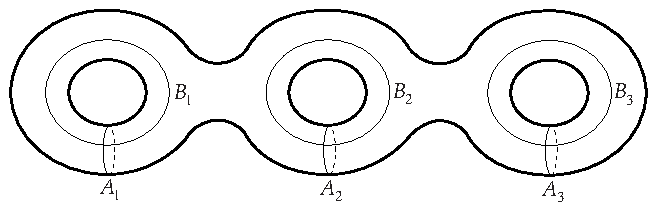
\includegraphics[width=0.8\linewidth]{figures/fig_9_1.pdf}
 \caption{$A$サイクルと$B$サイクルを描いた種数3の曲面。}\label{fig:9.1}
\end{figure}
\subsubsection*{Fuchsian群}
この構成では、まず世界面の計量を考える。Weyl変換によって世界面の曲率$R$を常に定数にできる、という定理がある。種数ゼロでは丸い球面、種数1では平坦なトーラス、高種数では一定の負曲率をもつ曲面が得られる。これらの単連結被覆空間も、同様に一定の曲率をもつ。このような単連結空間はちょうど3つある。丸い球面そのもの、平坦な平面（トーラスの被覆空間）、および計量
\begin{equation}
 ds^2=\frac{dz\,d\bar z}{(\operatorname{Im}z)^2}
 \tag{9.2.3}\label{eq:9.2.3}
\end{equation}
をもつ上半平面である。最後のものは、種数$g\geq2$のすべての曲面の被覆空間である。

これに対応して、種数$g\geq2$のすべての曲面は、上半平面をある離散群の作用で割ることによって得られる。この群の元は計量\hyperref[eq:9.2.3]{(9.2.3)}の等長変換でなければならず、これらの等長変換は実係数のMöbius変換$PSL(2,\mathbb R)$にほかならない。図\ref{fig:9.1}は、各ハンドルに$A$サイクルと$B$サイクルという閉曲線を描いた種数3の曲面を示している。これらの曲線は、点に縮められないという意味で非自明である。いずれかの曲線を1周すると、被覆空間では元の点には戻らず、それと同一視される点の1つに戻る。したがって各サイクルには$PSL(2,\mathbb R)$の元が対応し、それらも$A_i$または$B_i$と記す。

$A$サイクルと$B$サイクルは、どの閉経路もこれらを次々につないだものと同値（ホモトピック）であるという意味で完全である。実際には少し過剰であり、経路
\begin{equation}
 (A_1B_1^{-1}A_1^{-1}B_1)(A_2B_2^{-1}A_2^{-1}B_2)
 \cdots(A_gB_g^{-1}A_g^{-1}B_g)
 \tag{9.2.4}\label{eq:9.2.4}
\end{equation}
は1点に縮められるので、対応する積は恒等元でなければならない。モジュライを数えると、$PSL(2,\mathbb R)$の各元に3個の実パラメータがあって$6g$個となり、制約\hyperref[eq:9.2.4]{(9.2.4)}から3個、さらに$PSL(2,\mathbb R)$による全体の共役変換が同値な曲面を与えることから3個を引いて、合計$6g-6$個となる。

SchottkyとFuchsianのパラメータ表示は似ているが、性質はかなり異なる。とくに後者では複素構造がずっと見えにくく、それに応じて超弦への拡張も単純ではない。

\subsubsection*{周期行列}
トーラスのモジュラス$\tau$には、種数$g$において$g\times g$行列への自然な一般化がある。それを見るには、まずAbel微分、すなわち正則1形式が必要である。これらは、複素座標で
\begin{equation}
 \partial_{\bar z}\omega_z=0,\qquad\omega_{\bar z}=0
 \tag{9.2.5}\label{eq:9.2.5}
\end{equation}
を満たす世界面上の場$\omega_a$である。このような場はちょうど$g$個あり、さらに共役の関係を満たすものが$g$個ある。これはRiemann--Rochの定理\hyperref[eq:5.3.22]{(5.3.22)}から従う。Abel微分\hyperref[eq:9.2.5]{(9.2.5)}とその共役は演算子$P_0^T$の核にほかならず、この演算子に対するRiemann--Rochの定理は
\begin{equation}
 \dim\ker P_0^T-\dim\ker P_0=-\chi=2g-2
 \tag{9.2.6}\label{eq:9.2.6}
\end{equation}
である。演算子$P_0$は$h=0$のスカラー場$c,\tilde c$に作用するため、通常の勾配に帰着する。これには常に2つのゼロモード（$c=\text{定数}$または$\tilde c=\text{定数}$）があるので、$\dim\ker P_0^T=2g$となる。

1形式の線積分は座標不変な量である。したがってAbel微分の自然な基底は、
\begin{equation}
 \oint_{A_i}dz\,\omega_{zj}=\delta_{ij}
 \tag{9.2.7}\label{eq:9.2.7}
\end{equation}
によって定義される$\omega_{zi}$、$i=1,\ldots,g$である。すると周期行列
\begin{equation}
 \tau_{ij}=\oint_{B_i}dz\,\omega_{zj}
 \tag{9.2.8}\label{eq:9.2.8}
\end{equation}
が曲面の複素構造を特徴づける。種数1では$\omega_z$が定数なので、これは通常の$\tau$である。

$\tau_{ij}$が対称であることを示せるので、複素パラメータは$\tfrac12g(g+1)$個ある。$g=1,2,3$ではこれは複素モジュライの個数と等しいが、$g\geq4$ではそれより多い。したがって、すべての周期行列がRiemann面に対応するわけではない。テータ関数\hyperref[eq:7.2.36]{(7.2.36)}には自然な種数$g$への一般化があり、$\tau$は周期行列に、$\nu,n,a,b$は$g$成分ベクトルになる。

\subsubsection*{超楕円曲面}
ときに有用な別の記述を示そう。座標$z,y$をもつ空間$S_2\times S_2$を考える。複素パラメータ$Z_i$に対して、方程式
\begin{equation}
 y^2=\prod_{i=1}^{2k}(z-Z_i)
 \tag{9.2.9}\label{eq:9.2.9}
\end{equation}
で与えられる2次元部分多様体を考える。$z$座標に射影すると、$k$本の分岐切断を介してつながった2枚のシートがある。これによって$g=k-1$個のハンドルをもつ曲面ができる。分岐点は$z$に射影すると特異だが、曲面\hyperref[eq:9.2.9]{(9.2.9)}全体はそこで非特異であり、$y$が局所的によい座標となる。

曲面は$2k$個の複素数$Z_i$に依存するが、ここでもMöbius変換によってそのうち3個が冗長となり、$2k-3=2g-1$個の複素パラメータが残る。$g=1,2$ではこれはモジュライの数と等しいが、$g\geq3$ではモジュライの数のほうが多く、特別な曲面だけが\hyperref[eq:9.2.9]{(9.2.9)}の形をもつ。これらを超楕円曲面という。

\subsectionlink{世界面の縫い合わせと切断}\label{sec:9.3}
弦の振幅を解析するうえで有用なのは、高種数と低種数の振幅の間の関係である。その中心となるのが、低種数の曲面から高種数の曲面を作るための配管接合（plumbing fixture）である。あるパッチで座標$z_1$をもつ世界面$M_1$と、あるパッチで座標$z_2$をもつ世界面$M_2$を考える。これらを次のように接合して、新しい世界面$M$を作れる。$q$を複素パラメータとする。小さな$\epsilon$をとり、$M_1$から円板$|z_1|<(1-\epsilon)|q|^{1/2}$を、$M_2$から円板$|z_2|<(1-\epsilon)|q|^{1/2}$を切り取る。次に、
\begin{equation}
 z_1z_2=q
 \tag{9.3.1}\label{eq:9.3.1}
\end{equation}
を満たす点の対を同一視して、1つの曲面を作る。これを図\ref{fig:9.2}に示す。環状領域
\begin{equation}
 (1-\epsilon)^{-1}|q|^{1/2}>|z_1|>(1-\epsilon)|q|^{1/2}
 \tag{9.3.2}\label{eq:9.3.2}
\end{equation}
は図示したように縫い合わされる。この構成を表す記法の1つが
\begin{equation}
 M=M_1\infty M_2(z_1,z_2,q)
 \tag{9.3.3}\label{eq:9.3.3}
\end{equation}
である。この記法は、得られる曲面が局所座標の選択に依存することを強調している。異なる局所座標$z'_1,z'_2$を選べば、切り取る円が異なるため、接合した曲面も一般に異なる。2つのパッチが、単一の曲面$M_0$の異なる部分にあってもよい。その場合、配管接合による構成は曲面にハンドルを1つ加える。これを
\begin{equation}
 M=M_0 8(z_1,z_2,q)
 \tag{9.3.4}\label{eq:9.3.4}
\end{equation}
と記す。記号「$\infty$」と「$8$」は、2つの縫い合わせの過程を描き表す意図で用いている。実際にはパラメータ$q$は不要であり、$z'_1=z_1q^{-1/2}$、$z'_2=z_2q^{-1/2}$、$q'=1$とすると同値な曲面が得られる。座標パッチを固定したまま、$q$の関数としての振る舞いを論じるために$q$を導入すると便利なのである。

\begin{figure}[htbp]
 \centering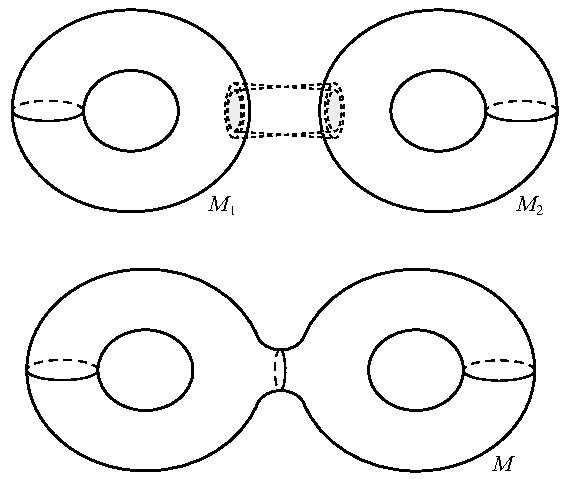
\includegraphics[width=0.8\linewidth]{figures/fig_9_2.pdf}
 \caption{2つの世界面のそれぞれから円板（網掛け部分）を取り除き、破線で示したように縁を貼り合わせて接合する。}\label{fig:9.2}
\end{figure}
この構成を逆にたどることもできる。任意のRiemann面$M$と、その上の自己交差しない任意の曲線$C$が与えられると、$C$の近傍で、$C$が$|z_1|=|z_2|=|q|^{1/2}$となる正則座標$z_1=z_2^{-1}$を常に見つけられる。$C$に沿って切断し（同一視$z_1z_2=q$を解き）、円板$|z_1|<|q|^{1/2}$と$|z_2|<|q|^{1/2}$を貼り込むと、$M_1$と$M_2$（または$M_0$）が得られる。縫い合わせ操作を行えば、これらから$M$を再構成できる。$C$に沿った切断によって曲面が非連結になるかどうかに応じて、操作は\hyperref[eq:9.3.3]{(9.3.3)}または\hyperref[eq:9.3.4]{(9.3.4)}となる。

図\ref{fig:9.2}の種数2の例で、$q\ll1$の場合を考えよう。図\ref{fig:9.3}(a)はこの場合の$M$を示している。重なり領域では、計量を$dz_1d\bar z_1$と$dz_2d\bar z_2$の間で滑らかに補間している。曲面は$|q|^{1/2}$程度の半径までくびれる。Weyl変換により、図\ref{fig:9.3}(b)に示すように半径が1程度に保たれる計量をとれる。Weyl変換は等方的に作用するため、ハンドルの長さが$-\ln|q|$程度まで大きくなる。ハンドル領域$|z_1|<1$、$|z_2|<1$は円筒
\begin{equation}
 \ln|q|<\operatorname{Im}w<0,\qquad w\cong w+2\pi
 \tag{9.3.5}\label{eq:9.3.5}
\end{equation}
と同値であり、$z_1=\exp(-iw)$、$z_2=q\exp(iw)$である。図\ref{fig:9.3}(c)は同じ曲面のもう1つの表現を示す。小さなハンドルを囲む環状領域$O(|q|)<|z|<O(1)$は、図\ref{fig:9.3}(b)の長い円筒と共形同値である。図\ref{fig:9.3}(a)から見ると、これは$M_2$全体を縮小するWeyl変換を行ったものと考えられる。

\begin{figure}[htbp]
 \centering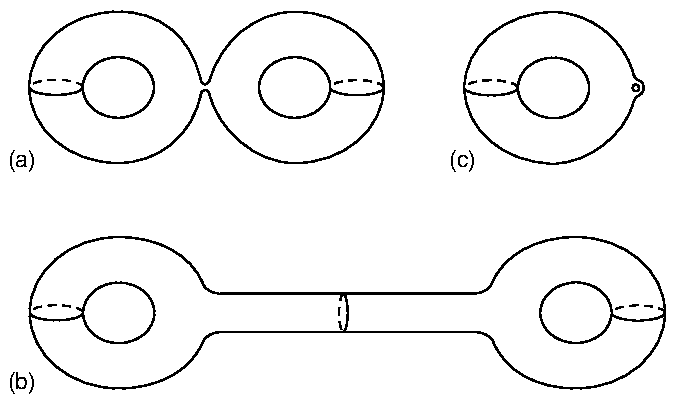
\includegraphics[width=0.8\linewidth]{figures/fig_9_3.pdf}
 \caption{サイクルが退化する種数2の曲面の3つの表現。}\label{fig:9.3}
\end{figure}
いずれの描像でも、$q\to0$極限で曲面が特別なものになることは明らかである。ハンドルがくびれる、または退化するという。これはモジュライ空間の境界の一例である。どのような発散もそこから生じるはずなので、モジュライ空間の境界は重要である。実際、すべての境界が、1つ以上のハンドルがくびれるこの形であることを見る。種数2の曲面では、単一のハンドルが退化する仕方がもう1つあり、$A$サイクルまたは$B$サイクルの1つがくびれる場合である。これは、2つのトーラスから「$\infty$」操作で作る代わりに、単一のトーラスから「$8$」操作で種数2の曲面を作り、$q\to0$とすることに対応する。

切断操作を繰り返すと、あらゆるRiemann面を3つの穿孔をもつ球面へと分解できる、という有用な事実がある。穿孔とは、指定された点とその近傍で定めた複素座標のことであり、配管接合を縫い込むために必要なデータである。言い換えると、あらゆるRiemann面は3つの穿孔をもつ球面を縫い合わせて構成できる。たとえば図\ref{fig:9.4}は、4つの頂点演算子をもつ種数2の曲面を構成する多数の方法のうち3つを示している。縫い合わせ操作ごとに複素モジュラス$q$が1つあり、図\ref{fig:9.4}の各構成では合計7個となる。これらは、種数2の曲面の$3g-3=3$個の複素モジュライと、4つの演算子の位置に対応する。

\begin{figure}[htbp]
 \centering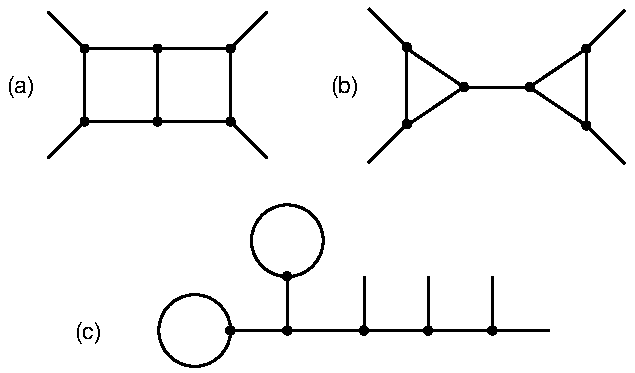
\includegraphics[width=0.8\linewidth]{figures/fig_9_4.pdf}
 \caption{4つの演算子をもつ種数2の曲面の、縫い合わせによる構成例。各頂点は3つの穿孔をもつ球面、各内線は配管接合による構成、各外線は頂点演算子を表す。}\label{fig:9.4}
\end{figure}
\subsubsection*{グラフによる分解}
図\ref{fig:9.4}のグラフはFeynman図を思わせる。ここでモジュライ空間のFeynman図に似た分解を述べよう。頂点は図\ref{fig:9.4}よりもかなり複雑で、任意の数の外線をもち、弦のループによる内部補正も含む。この構成の目的は、モジュライ空間の境界の性質を明示することにある。

主張は、モジュライ空間上の積分がFeynmanグラフの和で与えられる、というものである。グラフの各内部伝播関数は縫い合わせ操作を表し、縫い合わせパラメータ$q$を$|q|<1$のような標準的な領域で積分する。$n$点頂点は$n$個の穿孔をもつRiemann面を表す。後で見るように、頂点に含まれる曲面についてはモジュライ空間のある内部領域で積分し、さらに種数について和をとらなければならない。縫い合わせ操作は、縫い合わせる各点の特定の複素座標を参照するので、頂点の定義には各点での座標の選択も含めなければならない。$n$点頂点に現れる種数$g$のRiemann面の集合を$\mathcal V_{g,n}$と記す。外線は頂点演算子を表す。

この構成を具体的に示そう。3点頂点$\mathcal V_{0,3}$から始める。図\ref{fig:9.5}では、指定された3点と3つの縫い合わせ円をもつ球面として示してある。縫い合わせ円とは、それぞれの点に対応する複素座標での単位円である。この頂点を2つとり、それぞれから縫い合わせ円の1つの内部を取り除き、それらを円筒の両端に縫い合わせると、4点をもつ球面ができる。これは配管接合による構成と同値である。図\ref{fig:9.6}(a)のFeynmanグラフがこれに対応し、円筒の長さは、円周を$2\pi$に規格化すると$-\ln|q|$となる。$|q|<1$を積分し、他の2つのチャネルについて和をとっても、図\ref{fig:9.6}(b)に示すように、4点をもつ球面の積分領域の一部しか得られない。網掛けされた領域は含まれるが、網掛けのない内部領域は取り残される。

\begin{figure}[htbp]
 \centering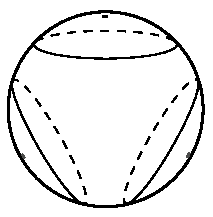
\includegraphics[width=0.65\linewidth]{figures/fig_9_5.pdf}
 \caption{球面上の3つの指定点と3つの縫い合わせ円をもつ、弦の3次頂点。}\label{fig:9.5}
\end{figure}
\begin{figure}[htbp]
 \centering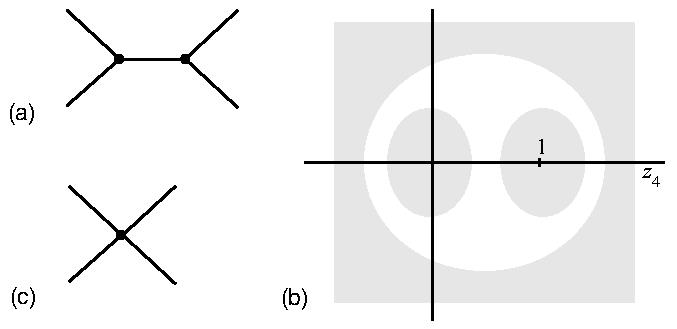
\includegraphics[width=0.8\linewidth]{figures/fig_9_6.pdf}
 \caption{(a) 4つの頂点演算子をもつ球面の構成。(b) このグラフが覆う$z$平面の領域。(c) 正しい振幅を得るために追加が必要な頂点。4つの穿孔をもつ球面を網掛けのない領域で積分する。}\label{fig:9.6}
\end{figure}
さらに具体化しよう。3次頂点について、球面上の点を標準的な位置$0,1,\infty$に置き、それぞれで座標系$z^{(0)},z^{(1)},z^{(\infty)}$を選ぶと、3つの縫い合わせ円は$|z^{(0,1,\infty)}|=1$となる。頂点が対称になるように、この選択は頂点演算子を置換する6つのMöbius変換の下で、位相を除いて不変でなければならない。可能な選択は多数あり、たとえば任意の定数$a$に対して
\begin{equation}
 z^{(0)}=\frac{az}{z-2},\qquad
 z^{(1)}=\frac{a(z-1)}{z+1},\qquad
 z^{(\infty)}=\frac{a}{2z-1}
 \tag{9.3.6}\label{eq:9.3.6}
\end{equation}
とできる。$a\geq3$では縫い合わせ円が重ならず、すべての$q\leq1$について配管接合が適切な曲面を与えることが保証される。読者が確かめられるように、2つの球面の$z^{(\infty)}$パッチと$z'^{(0)}$パッチをパラメータ$q$で縫い合わせると、$0,1,\tfrac12(1+a^2/q),\tfrac12(1-a^2/q)$に頂点演算子をもつ球面が得られる。これはMöbius変換により、$0,1,\infty$および
\begin{equation}
 z_4=\frac{(q-a^2)^2}{4a^2q}
 \tag{9.3.7}\label{eq:9.3.7}
\end{equation}
に頂点演算子をもつ球面と同値である。$q$が単位円板を走ると、$z_4$は図\ref{fig:9.6}(b)の外側の網掛け領域を覆う。外部の頂点演算子を置換すると、残りの2つの領域が得られる。$a$を小さくして網掛け領域を広げようとしても、やがて領域が重なって一部の曲面を二重に数える一方、依然として生成されない曲面が残る。これらが平面を過不足なく埋め尽くすことはない。そのため、4つの指定点をもつ球面を$z$平面の網掛けのない部分で積分した、明示的な4点頂点$\mathcal V_{0,4}$を加える必要がある。これだけでは$\mathcal V_{0,4}$の定義は完全ではない。$z_4$の各値に対し、各穿孔での座標も選ばなければならないからである。網掛け領域とそうでない領域の境界で滑らかにつながるように、その選択を行うことが常に可能である。図\ref{fig:9.6}(a)のFeynmanグラフはすべての漸近領域$z_4\to0,1,\infty$を含む一方、4点頂点には非退化な曲面だけが含まれることに注意しよう。したがって極限での振る舞いは、配管接合の$q\to0$極限によって明示的に与えられる。これがこの構成の有用な理由である。

別の例として、1つの頂点の2つの円を円筒の両端に縫い合わせると、1つの頂点演算子をもつトーラスができる。これはトーラスのモジュライ空間の$\operatorname{Im}\tau\to\infty$極限を覆うが、内部領域が取り残されるため、頂点領域$\mathcal V_{1,1}$として別途加えなければならない。

この構成は帰納的に拡張できる。縫い合わせ操作は、パラメータ
\begin{equation}
 r=3g+n-2
 \tag{9.3.8}\label{eq:9.3.8}
\end{equation}
を常に増加させる。出発点の3つの穿孔をもつ球面、頂点$\mathcal V_{0,3}$では$r=1$である。$8$操作は$r=r_0+1$を、$\infty$操作は$r=r_1+r_2$を与える。したがって$\mathcal V_{0,4}$と$\mathcal V_{1,1}$はいずれも$r=2$である。$r$について帰納的に$\mathcal V_{g,n}$を構成でき、それによって主張どおりモジュライ空間を覆えることが示されている。

より明示的な構成は次のとおりである（証明は参考文献にある）。任意のRiemann面には一意な最小面積計量が存在する。これは、すべての非自明な閉曲線（連続的に1点に縮められない曲線）の長さが少なくとも$2\pi$であるという制約のもとで、面積を最小にする計量として定義される。曲面上のすべての点は、長さがちょうど$2\pi$の非自明な閉曲線である、制約を飽和する測地線の少なくとも1つの上にある。互いに連続的に変形できる、すなわちホモトピー同値な、制約を飽和する測地線どうしは交差できない。ホモトピー同値な飽和測地線の各集合は、曲面上に帯（位相的には環）を作る。異なる帯は曲面を完全に覆い、互いに重なっていてもよい。帯の高さ$h$は、その境界となる2本の測地線の間の最短距離として定義する。穿孔のまわりを回る曲線を非自明とみなすと定めれば、最小面積計量の考えを穿孔のある曲面へも拡張できる。穿孔の近くでの最小面積計量は$dz\,d\bar z/z\bar z$という形であり、半径$2\pi$の半無限円筒である。したがって帯には2種類ある。曲面内部にある有限の帯と、穿孔を中心とし、曲面内部で終わる半無限の帯である。

この構成での$\mathcal V_{g,n}$を記述できるようになった。$n$個の穿孔をもつすべてのRiemann面をとる。ただし、最小面積計量で測ったすべての内部の帯の高さが$2\pi$未満であることを要求する。半無限円筒を、長さ$\pi$の短い管を残して切り落とし、その端に頂点演算子をもつ通常の単位円板を貼り込む。これらの頂点を用いると、Feynmanグラフの和はモジュライ空間をちょうど1回覆う。これらの最小面積曲面を縫い合わせたものも、最小面積曲面になることを示せる。高さ$2\pi$未満の帯は、頂点に明示的に含まれている。高さ$2\pi$より大きい帯は、短い管を縫い合わせる操作で生成される。その高さは、短い管からの$2\pi$に、配管接合からの$-\ln|q|$を加えたものであり、$q$を積分すると$2\pi$から$\infty$までを走る。長さの下限と高さの上限の制約により、退化する曲面は頂点に現れないことが保証される。したがって、それらは主張どおり、1つ以上の$q$がゼロになることによってのみ生じる。

\subsectionlink{CFTの縫い合わせと切断}\label{sec:9.4}
高種数のRiemann面を、低種数の曲面を縫い合わせて作るものとして記述した。経路積分の縫い合わせの性質を用いると、高種数の曲面上のCFTも同様に低次の振幅と関係づけられる。この関係を図\ref{fig:9.7}に描いてある。話を明確にするため、まず$q=1$の場合を論じよう。境界状態の完全系を挿入して、$M$上の経路積分を円$|z_1|=|z_2|=1$に沿って切り開く。次に、各境界状態を対応する局所演算子をもつ円板で置き換えると、切断前の世界面$M_1,M_2$が残る。結果の正確な形は
\begin{equation}
 \langle\cdots_1\cdots_2\rangle_M
 =\sum_{ij}\left\langle\cdots_1\mathcal A_i^{(z_1)}\right\rangle_{M_1}
 \mathsf G^{ij}\left\langle\mathcal A_j^{(z_2)}\cdots_2\right\rangle_{M_2}
 \tag{9.4.1}\label{eq:9.4.1}
\end{equation}
である。$M_1$上の任意の追加の挿入$\cdots_1$と、$M_2$上の任意の追加の挿入$\cdots_2$を許している。もちろん、これらは切断する円$|z_1|=1$および$|z_2|=1$の外側になければならない。基底には特定の正規直交条件を課していない。適切な逆計量$\mathsf G^{ij}$は、これから決める。ハンドルを置き換える挿入$\mathcal A_i,\mathcal A_j$は、それぞれ$z_1,z_2$座標系の原点にあるものとする。

\begin{figure}[htbp]
 \centering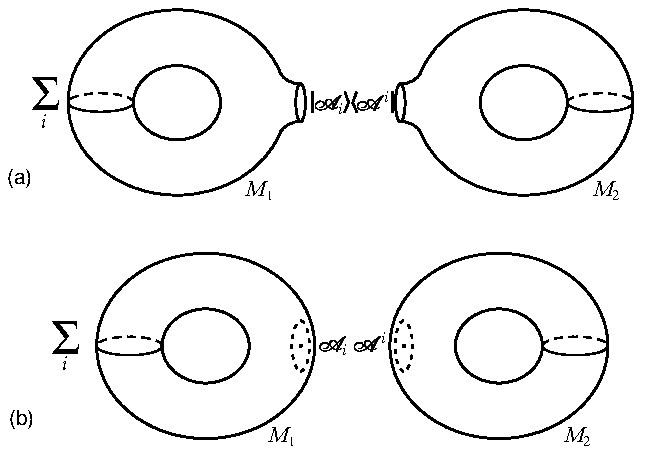
\includegraphics[width=0.8\linewidth]{figures/fig_9_7.pdf}
 \caption{(a) 境界状態の完全系を挿入して、$M$上の経路積分を切り開く。(b) 各状態を、局所演算子をもつ円板で置き換える。}\label{fig:9.7}
\end{figure}
次に、$M_2$が球面で、縫い合わせ座標$z_2$が$u$、$\cdots_2$が$z=0$にあるある局所演算子$\mathcal A_k$である場合を考えよう。配管接合から$z_1u=1$、球面から$zu=1$という同一視があるので、$z_1=z$を縫い合わせ領域全体へそのまま延長できる。縫い合わせた曲面$M$は、$z_1=0$に演算子$\mathcal A_k$を加えた$M_1$と同じである。すると式\hyperref[eq:9.4.1]{(9.4.1)}は
\begin{equation}
 \left\langle\cdots_1\mathcal A_k^{(z_1)}\right\rangle_{M_1}
 =\sum_{ij}\left\langle\cdots_1\mathcal A_i^{(z_1)}\right\rangle_{M_1}
 \mathsf G^{ij}\left\langle\mathcal A_j^{(u)}\mathcal A_k^{(z)}\right\rangle_{S_2}
 \tag{9.4.2}\label{eq:9.4.2}
\end{equation}
となる。2点関数$\langle\mathcal A_j^{(u)}\mathcal A_k^{(z)}\rangle_{S_2}$は、内積$\langle\!\langle j|k\rangle=\mathcal G_{jk}$にほかならない。したがって式\hyperref[eq:9.4.2]{(9.4.2)}から
\begin{equation}
 \mathsf G^{ij}\mathcal G_{jk}=\delta^i_k
 \tag{9.4.3}\label{eq:9.4.3}
\end{equation}
すなわち
\begin{equation}
 \mathsf G^{ij}=\mathcal G^{ij}
 \tag{9.4.4}\label{eq:9.4.4}
\end{equation}
が従う。つまり、球面上の2点関数によって定義される内積こそが、縫い合わせに対する正しい内積である。これで、$M_2$が任意の局所演算子をもつ球面である場合に、関係\hyperref[eq:9.4.1]{(9.4.1)}を導いた。状態・演算子同型により、任意の境界状態がこの方法で得られる。経路積分は局所的なので、結果は縫い合わせの領域だけに依存し、曲面の残りの部分には依存しない。したがって、任意の$M_2$および$\cdots_2$について成り立つ。

パラメータ$q$による縫い合わせは、$q=1$で局所座標$z_1$および$z'_2=z_2/q$を用いて縫い合わせることと同じである。したがって、$\mathcal A_j$をプライム付き座標系で表した式\hyperref[eq:9.4.1]{(9.4.1)}が得られ、$z_2$へ戻す共形変換から追加の因子
\begin{equation}
 \mathcal A_j^{(z'_2)}=q^{h_j}\bar q^{\tilde h_j}\mathcal A_j^{(z_2)}
 \tag{9.4.5}\label{eq:9.4.5}
\end{equation}
が生じる。結果は
\begin{equation}
 \langle\cdots_1\cdots_2\rangle_M
 =\sum_{ij}q^{h_j}\bar q^{\tilde h_j}
 \left\langle\cdots_1\mathcal A_i^{(z_1)}\right\rangle_{M_1}
 \mathcal G^{ij}\left\langle\mathcal A_j^{(z_2)}\cdots_2\right\rangle_{M_2}
 \tag{9.4.6}\label{eq:9.4.6}
\end{equation}
であり、共形ウェイトについて対角な基底を選んでいる。「$8$」操作の場合にも、$M$と$M_0$上の経路積分は同様に関係づけられる。
\begin{equation}
 \langle\cdots\rangle_M
 =\sum_{ij}q^{h_j}\bar q^{\tilde h_j}\mathcal G^{ij}
 \left\langle\cdots\mathcal A_i^{(z_1)}\mathcal A_j^{(z_2)}\right\rangle_{M_0}.
 \tag{9.4.7}\label{eq:9.4.7}
\end{equation}

1つ以上のハンドルの$q\to0$極限で与えられる、モジュライ空間の境界を改めて考えると興味深い。最も低い共形ウェイトの演算子が振る舞いを支配することがわかる。結果\hyperref[eq:9.4.6]{(9.4.6)}と\hyperref[eq:9.4.7]{(9.4.7)}はOPEに似ており、実際、$M_2$が球面で「$\cdots_2$」が1対の頂点演算子である場合、\hyperref[eq:9.4.6]{(9.4.6)}はOPEに帰着する。この類似は、極限を小さなハンドルの挿入として表す図\ref{fig:9.3}(c)からとくに明瞭にわかる。縫い合わせ関係は、演算子の積だけでなく、小さなハンドルや、世界面上の小さな円の中に縫い込める任意の変形も、局所演算子の和と同値であることを示す。結果\hyperref[eq:9.4.6]{(9.4.6)}はOPEの美しい一般化である。$M_1$から見ると、$z_1=0$の近くに$M_2$の小さな複製が貼り込まれている。これは、$\langle\mathcal A^i\cdots_2\rangle_{M_2}$を係数関数として、局所演算子$\mathcal A_i$で展開できる。$M_2$から見ると、$z_2=0$の近くに$M_1$の小さな複製が貼り込まれており、係数関数$\langle\cdots_1\mathcal A_i\rangle_{M_1}$を用いて局所演算子$\mathcal A^i$で展開される。

あらゆるRiemann面は3つの穿孔をもつ球面へと分解できると論じた。したがって縫い合わせによる構成は、すべての振幅を球面上の3点振幅に関係づける。後者は本質的に演算子積係数であり、これらがCFTを定義するデータである。今後、CFTの間の多くの同値性に出会うことになる。すでに$T$双対性を見たが、ボソン化（第10章）も顕著な例である。縫い合わせによる構成は、2つの理論が同じであるための判定基準を与える。それは、状態（または局所演算子）の間に1対1の対応があり、OPEが一致することである。\footnote[1]{第2.5節の自由場の例のように、$T_{ab}$の役割を果たしうる$(2,0)$と$(0,2)$の場の組が複数ある場合には、そのうちどれがエネルギー運動量テンソルなのかを指定する必要がある。この選択が演算子の共形変換を決め、その変換は縫い合わせ関係に暗黙に入っていることに注意しよう。}実際、第15章で示すように、一次場の演算子積だけで他のすべての場の演算子積が決まる。

この見方をさらに調べよう。曲面は多くの異なる曲線の組に沿って切断できるので、縫い合わせ関係が常に$M$上の期待値に対して同じ結果を与えるための整合性条件がなければならない。まず、切断曲線$C$の無限小変化を考える。$M$を不変に保つ一般の無限小変化は、縫い合わせに用いる座標の無限小変化
\begin{align}
 z'_1&=z_1+\sum_{n=-\infty}^{\infty}\epsilon_n z_1^{n+1},
 \tag{9.4.8a}\label{eq:9.4.8a}\\
 z'_2&=z_2-\sum_{n=-\infty}^{\infty}\epsilon_{-n}q^{-n}z_2^{n+1}
 \tag{9.4.8b}\label{eq:9.4.8b}
\end{align}
によって得られる。すると、縫い合わせて得られる式の差は
\begin{equation}
 \begin{aligned}
 &\mathcal A_i^{(z'_1)}\mathcal G^{ij}\mathcal A_j^{(z'_2)}
 -\mathcal A_i^{(z_1)}\mathcal G^{ij}\mathcal A_j^{(z_2)}\\
 &\quad=-\sum_{n=-\infty}^{\infty}\epsilon_n
 \Bigl[L_n\cdot\mathcal A_i^{(z_1)}\mathcal G^{ij}\mathcal A_j^{(z_2)}
 -\mathcal A_i^{(z_1)}\mathcal G^{ij}L_{-n}\cdot\mathcal A_j^{(z_2)}\Bigr]
 +(\mathrm{anti})
 \end{aligned}
 \tag{9.4.9}\label{eq:9.4.9}
\end{equation}
に比例する。ここでは共形変換\hyperref[eq:2.9.6]{(2.9.6)}を用いた。「anti」は、$\epsilon_n\to\epsilon_n^*$、$L_n\to\tilde L_n$と置き換えた同じ形を表す。括弧内の量が消えることは、式\hyperref[eq:9.4.4]{(9.4.4)}の導出と同様の議論によって示せる。これは、生成子を定義する周回積分を、縫い合わせたハンドルを通して引き抜ける、ということにほかならない。$L_n$から$L_{-n}$への変化は座標の反転による。保存電荷に対する他のすべての周回積分も、同様に通り抜けさせられる。

連続変形で結ばれない曲線の組もある。球面上の4点振幅は、異なる演算子の対を囲む曲線に沿って切断することで、3点関数を用いて書ける。異なる縫い合わせの間で結果が等しいことは、図\ref{fig:2.8}に示したOPEの結合律である。

もう1つの例はトーラスである。$A$サイクル、$B$サイクル、あるいは他の任意の自己交差しない閉曲線に沿って切断することで、トーラスを球面へと帰着できる。同一視を伴う平面の言葉でいうと、$(\sigma^1,\sigma^2)=(0,0)$から出発する閉曲線$C$は、それと同一視される点
\begin{equation}
 2\pi(m,n)
 \tag{9.4.10}\label{eq:9.4.10}
\end{equation}
で終わらなければならない。同じ$m,n$の値をもつすべての曲線は互いに連続的に変形できるので、異なる$m,n$の曲線で縫い合わせる場合の関係を考えればよい。非自明で自己交差しない曲線の場合、$m,n$は互いに素でなければならないことを示せる。したがって、$mp-nq=1$を満たす整数$p,q$が存在する。するとモジュラー変換
\begin{equation}
 (\sigma^1,\sigma^2)=(\sigma'^{1},\sigma'^{2})
 \begin{bmatrix}m&n\\q&p\end{bmatrix}
 \tag{9.4.11}\label{eq:9.4.11}
\end{equation}
があり、曲線$C$は
\begin{equation}
 (\sigma'^{1},\sigma'^{2})=2\pi(1,0)
 \tag{9.4.12}\label{eq:9.4.12}
\end{equation}
へ戻る。これは$A$サイクルである。したがって、一般の非自明で自己交差しない曲線に沿って切断することは、モジュラー同値な$\tau$の値に対して$A$サイクルに沿って切断することと同値である。ゆえに、縫い合わせによる構成の整合性はモジュラー不変性と同値である。

縫い合わせ曲線の任意の組は、2種類の操作を繰り返すことで、他の任意の組へ移せる。その操作は、球面上の4点の結合律変換と、1つの頂点演算子をもつトーラス上のモジュラー変換である。図\ref{fig:9.4}を見ると、これがもっともらしいことがわかる。たとえば図\ref{fig:9.4}(a)と図\ref{fig:9.4}(b)は1つの結合律条件で結ばれる。結合律を繰り返し適用すると、すべてのループが1ループ1点関数で表された図\ref{fig:9.4}(c)の形に縫い合わせを変えられる。したがって、これらが、任意の演算子積係数の集合が矛盾のない共形場理論を定義するための条件である。双対性の制約を解くこの研究方針は、共形ブートストラップと呼ばれる。第15章で論じるように、追加の制約を導入した場合にのみ実行されている。

本節の考察はすべて、境界をもつ世界面にも拡張される。その場合、退化するハンドルに加えて、退化する帯が現れることもある。整合性条件はこの場合にも一般化されている。

